\section{Extending SyN for multi-modality images}

Let $I$, $J$ be two images defined over the domains $\Omega_{I}$, $\Omega_{J}$, respectively. Let $G$ be the set of
possible intensity values these images may take (e.g. $G=\left\lbrace 0,1,...,255\right\rbrace$). Our objective is to find two diffeomorphisms
$\Psi_{I}:\Omega_{I}\rightarrow \Omega_{R}$, $\Psi_{J}:\Omega_{J}\rightarrow \Omega_{R}$ such that the images get aligned in the reference space $\Omega_{R}$
after warping them under $\Psi_{I}^{-1}$ and $\Psi_{J}^{-1}$. In other words, for each point $u \in \Omega_{R}$, $I(\Psi_{I}^{-1}(u))$ ``corresponds to'' $J(\Psi_{J}^{-1}(u))$
(fig. \ref{fig:syn_overview}). We will model the intensity correspondence between the two images as a set of hidden variables. More precisely, we will assume that there exist transfer functions
$F_{I}, F_{J}:G \rightarrow G$ such that:\\
\begin{equation}\label{eq:SyNEM_gom_ref}
    \begin{array}{ccccc}
        I(\Psi_{I}^{-1}(u)) &=& F_{J}[J(\Psi_{J}^{-1}(u))] &+& \eta_{J}(u)\\
        J(\Psi_{J}^{-1}(u)) &=& F_{I}[I(\Psi_{I}^{-1}(u))] &+& \eta_{I}(u)
    \end{array}, u\in\Omega_{R},
\end{equation}
where $\eta_{I}, \eta_{J}$ are independent random fields of independent random variables, i.e. $\eta_{I}(u) \perp \eta_{I}(v)$,
$\eta_{J}(u) \perp \eta_{J}(v)$ and $\eta_{I}(u) \perp \eta_{J}(v) \forall u,v\in \Omega_{R}$. By defining the warped images $\tilde{I}(u) = I(\Psi_{I}^{-1}(u))$
and $\tilde{J}(u) = J(\Psi_{J}^{-1}(u)), u \in \Omega_{R}$ we can write

\begin{figure}[H]
\centering
\fbox{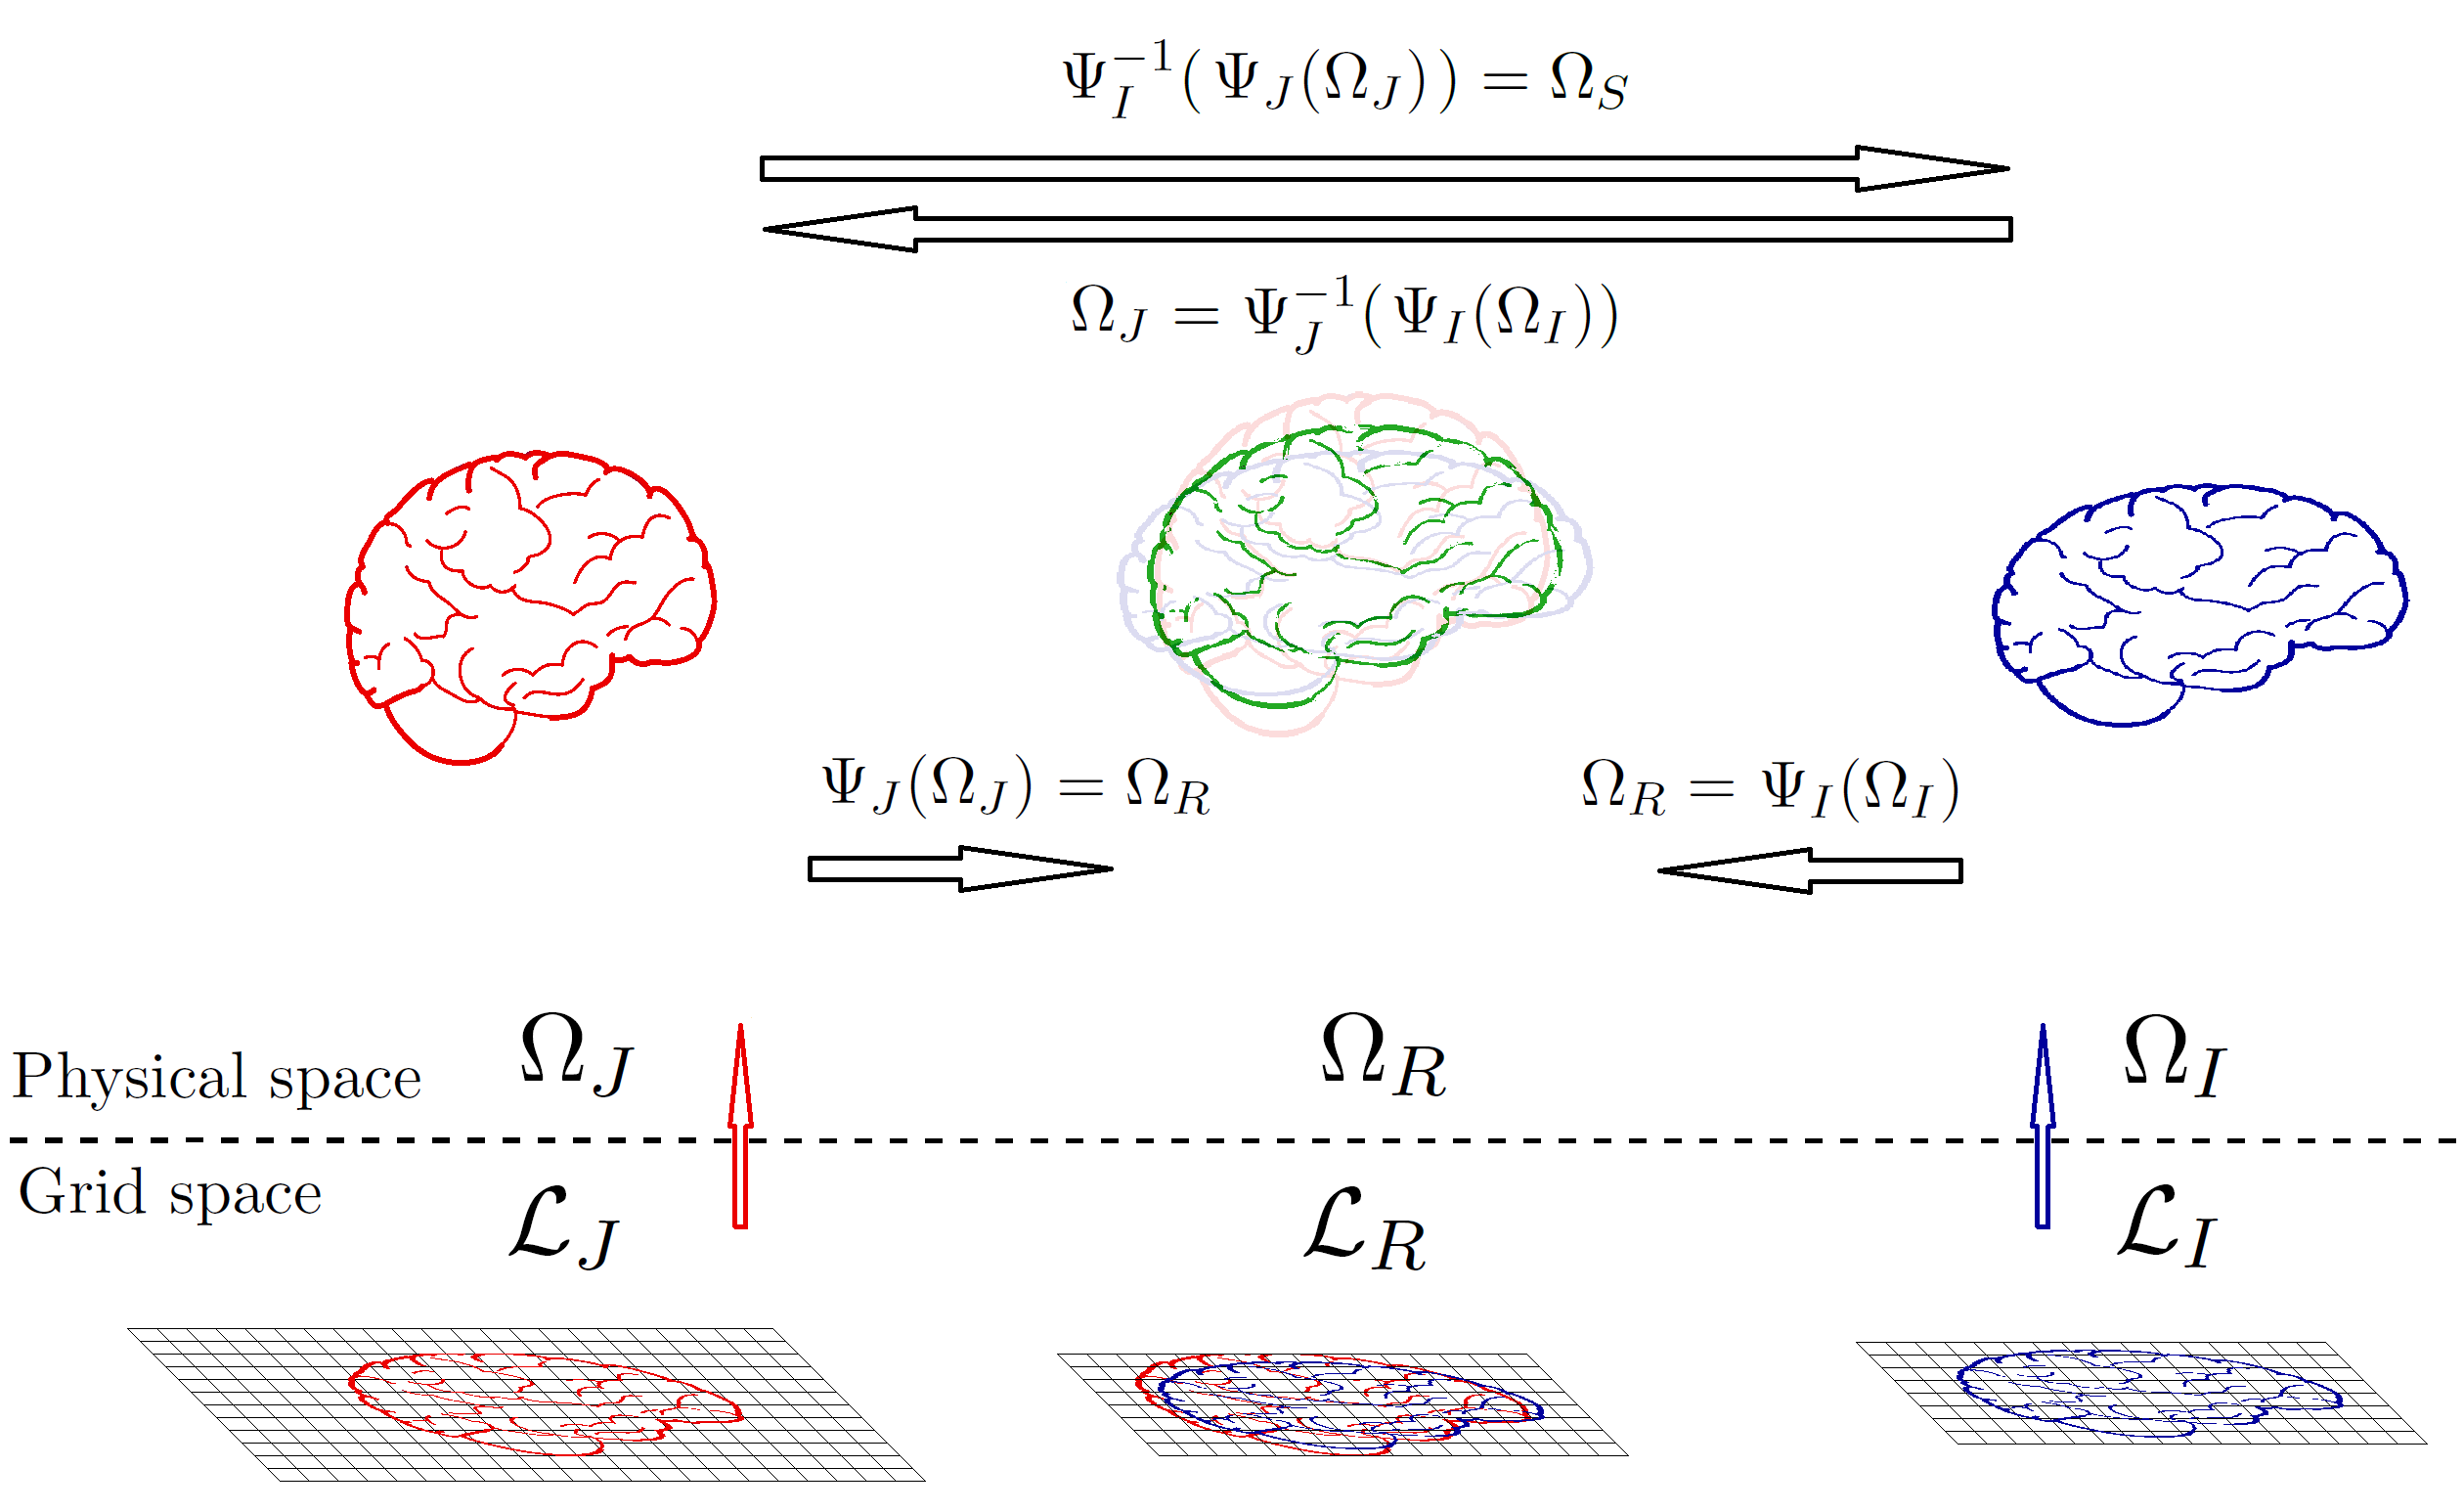
\includegraphics[width=1.0\linewidth]{./images/syn_overview.png}}
\caption{The SyN algorithm registers two input images by computing two diffeomorphisms that map the input images towards a common reference domain. The final
diffeomorphism is computed by composing the two partial diffeomorphisms.}
\label{fig:syn_overview}
\end{figure}

\begin{equation}\label{eq:SyNEM_gom_warped}
    \begin{array}{ccccc}
        \tilde{I}(u) &=& F_{J}[\tilde{J}(u)] &+& \eta_{J}(u)\\
        \tilde{J}(u) &=& F_{I}[\tilde{I}(u)] &+& \eta_{I}(u)
    \end{array}, u\in\Omega_{R},
\end{equation}
and now, both images are defined on the reference space. If we assume $\Psi_{I}$ and $\Psi_{J}$ are initial approximations to the true transformations
aligning $I$ and $J$, we are interested in computing two update diffeomorphisms (endomorphisms) \hbox{$\psi_{I}, \psi_{J} : \Omega_{R} \rightarrow \Omega_{R}$} such that

\begin{equation}\label{eq:SyNEM_gom_update}
    \begin{array}{ccccc}
    	\tilde{I}(\psi_{I}(u)) &=& F_{J}[\tilde{J}(u)] &+& \eta_{J}(u)\\
        \tilde{J}(\psi_{J}(u)) &=& F_{I}[\tilde{I}(u)] &+& \eta_{I}(u)
    \end{array}, u\in\Omega_{R}.
\end{equation}

By introducing the (unknown) sets of hidden variables $Y = \left\lbrace Y_{g}=F_{I}[g] : g\in G \right\rbrace$, $Z = \left\lbrace Z_g = F_{J}[g] : g \in G\right\rbrace$ we may
apply the EM algorithm to iteratively maximize the posterior distribution
$P(\Psi | \tilde{I}, \tilde{J}) = \frac{P(\tilde{I}, \tilde{J} | \Psi)P(\Psi)}{P(\tilde{I}, \tilde{J})}$ with respect to the transformations
$\Psi = (\psi_{I}, \psi_{J})$. The estimated diffeomorphisms at iteration $t$, $\Psi^{t} = \left( \psi_{I}^{t}, \psi_{J}^{t}\right)$ can be obtained from those at iteration
$t-1$ by maximizing, with respect to $\Psi$:
\begin{equation}
	Q(\Psi, \Psi^{t-1}) = E_{Y,Z}\left[\log \left( \frac{P(\tilde{I}, \tilde{J}, Y, Z|\Psi)P(\Psi)}{P(\tilde{I}, \tilde{J}, Y, Z)}\right) | \tilde{I}, \tilde{J}, \Psi^{t-1}\right].
\end{equation}
To evaluate this expected value, we need to integrate over all possible realizations $y, z$ of the hidden variables $Y, Z$ with respect to the conditional distribution $P(y,z| \tilde{I}, \tilde{J}, \Psi^{t-1})$:
\begin{equation}\label{eq:expected_value}
Q(\Psi, \Psi^{t-1}) = \int_{y,z} (U(\Psi, y, z) - K_1)dP(y,z| \tilde{I}, \tilde{J}, \Psi^{t-1})
\end{equation}
where $K_{1} =\log P(\tilde{I}, \tilde{J}, Y, Z)$ is a normalization constant (does not depend on $\Psi$) and
\begin{align}\label{eq:SyNEM_objective}
	U(\Psi, y, z) = \log P(\tilde{I}, \tilde{J}, y, z|\Psi) + \log P(\Psi)=\\
    \nonumber\sum_{g\in G} \sum_{x : \tilde{I}(x) = g} -\frac{\left(y_g - \tilde{J}(\psi_{I}(x))\right)^{2}}{\sigma_{I}(g)^{2}} + \lambda R(\psi_{I})+\\
    \nonumber\sum_{g\in G} \sum_{x : \tilde{J}(x) = g} -\frac{\left(z_g - \tilde{I}(\psi_{J}(x))\right)^{2}}{\sigma_{J}(g)^{2}} + \lambda R(\psi_{J}).
\end{align}
The regularization functional $R(\cdot)$ encode our prior knowledge about $\Psi$ by $\log P(\Psi) = \lambda \left( R(\psi_{I}) + R(\psi_{J})\right)$ where $\lambda > 0$ is a parameter controlling the amount of regularization.\\

If we assume $Y$ and $Z$ are independent, and their elements $Y_g$ and $Z_g$, $g\in G$ are independent from each other, then the density function $P(y,z| I, J, \Psi^{t-1})$ can be written as the product of two separate densities
\begin{equation}\label{eq:density_products}
    P(y,z| I, J, \Psi^{t-1}) = h_{Y}(y)h_{Z}(z) = \prod_{g\in G}h_{Y_g}(y_g) \prod_{g\in G}h_{Z_g}(z_g),
\end{equation}
and the expected value (eq. \ref{eq:expected_value}) can be written as
\begin{align}
    -K_{1}-\int\sum_{g\in G} \sum_{x : I(x) = g} \frac{\left(y_g - \tilde{J}(\psi_{I}(x))\right)^{2}}{\sigma_{I}(g)^{2}}d h_{Y}(y)-\\
    \nonumber\int\sum_{g\in G} \sum_{x : J(x) = g} \frac{\left(z_g - \tilde{I}(\psi_{J}(x))\right)^{2}}{\sigma_{J}(g)^{2}}d h_{Z}(z)
\end{align}
which can be further simplified (by using eq. \ref{eq:density_products} to split the densities $h_{Y}(y)$ and $h_{Z}(z)$ as products of individual densities for each intensity $g \in G$) as
\begin{align}
    -K_{1}-\sum_{g\in G} \sum_{x : I(x) = g} \int\frac{\left(r - \tilde{J}(\psi_{I}(x))\right)^{2}}{\sigma_{I}(g)^{2}}d h_{Y_g}(r)-\\
    \nonumber\sum_{g\in G} \sum_{x : J(x) = g} \int\frac{\left(s - \tilde{I}(\psi_{J}(x))\right)^{2}}{\sigma_{J}(g)^{2}}d h_{Z_g}(s)
\end{align}
now let $\bar{r}(g)$ and $\bar{s}(g)$ be the expected value of $Y_g$ and $Z_g$ given $I, J, \Psi^{t-1}$ respectively, then
\begin{align}
    &\int\left(r - \tilde{J}(\psi_{I}(x))\right)^{2}d h_{Y_g}(r) = &\\
    &\nonumber \int\left(r - \bar{r}(g) + \bar{r}(g) - \tilde{J}(\psi_{I}(x))\right)^{2}d h_{Y_g}(r) = &\\
    &\nonumber \sigma^{2}_{I}(g) + \int\left(\bar{r}(g) - \tilde{J}(\psi_{I}(x))\right)^{2}d h_{Y_g}(r) = &\\
    &\nonumber \sigma^{2}_{I}(g) + \left(\bar{r}(g) - \tilde{J}(\psi_{I}(x))\right)^{2}&
\end{align}
because $h_{Y_g}$ is a density function and we are integrating over its entire domain. Analogously:
\begin{align}
    \int\left(s - \tilde{I}(\psi_{J}(x))\right)^{2}d h_{Z_g}(s) = \sigma^{2}_{J}(g) + \left(\bar{s}(g) - \tilde{I}(\psi_{J}(x))\right)^{2}
\end{align}

Now let's denote by $\hat{\mu}_{I}(x) = \bar{r}(\tilde{I}(x))$, $\hat{\sigma}_{I}(x) = \sigma_{I}(\tilde{I}(x))$ and analogously
$\hat{\mu}_{J}(x) = \bar{s}(\tilde{J}(x))$, $\hat{\sigma}_{J}(x) = \sigma_{J}(\tilde{J}(x))$, in other words, we assign to each voxel $x$ from
$\tilde{I}$ the expected value $\bar{r}(g)$ corresponding to the intensity $g$ of $\tilde{I}$ at $x$ and denote it by $\hat{\mu}_{I}(x)$, assign
its corresponding variance and denote it by $\hat{\sigma_{I}}(x)$ and proceed analogously for $\hat{\mu}_{J}(x)$ and $\hat{\sigma}_{J}(x)$ using $J$.
Then, the expected value that needs to be maximized in the M-step of the EM algorithm (eq. \ref{eq:expected_value}) can be written as:
\begin{align}\label{eq:SyNEM_objective}
    -Q(\Psi, \Psi^{t-1}) = \sum_{x \in \Omega_{I}} \frac{(\hat{\mu}_{I}(x) - \tilde{J}(\psi_{I}(x)))^{2}}{\hat{\sigma}_{I}(x)} + \lambda R(\psi_{I}) + \\
    \nonumber\sum_{x \in \Omega_{J}} \frac{(\hat{\mu}_{J}(x) - \tilde{I}(\psi_{J}(x)))^{2}}{\hat{\sigma}_{J}(x)} + \lambda R(\psi_{J})
\end{align}

The main difficulty of directly minimizing eq. (\ref{eq:SyNEM_objective}) is that both similarity terms depend on both diffeomorphisms
$\psi_{I}$ and $\psi_{J}$ since $\tilde{J}(\psi_{I})$ depends on $\psi_{J}^{-1}$ and $\tilde{I}(\psi_{J})$ depends on $\psi_{I}^{-1}$, which implies that the
objective function must be optimized with respect to both diffeomorphisms simultaneously, which is very challenging because an explicit formula for the representation
of $\psi_{I}^{-1}$ and $\psi_{J}^{-1}$ in terms of the parameters of $\psi_{I}$ and $\psi_{J}$ may not be available or may be prohibitively costly to compute
\footnote{Diffeomorphisms are typically parameterized by displacement fields (a displacement vector for each voxel) and the problem of inverting a displacement field
has been subject of substantial research. All available methods for approximating displacement field inverses are iterative, see for example:
\cite{Chen2008}\cite{Avants2009}\cite{Christensen2001}\cite{Crum2007}\cite{Yan2010}}. To overcome this difficulty, the greedy SyN algorithm proposed by Avants et al.
\cite{Avants2011} uses the inverses at iteration $t-1$ to compute $\tilde{I}$ and $\tilde{J}$, then updates the direct transformations at iteration $t$ and updates the
inverses at iteration $t$ by inverting $\psi_{I}^{t}$ and $\psi_{J}^{t}$ using a variation of the fixed point algorithm proposed by Chen et al.\cite{Chen2008} (see
algorithm \ref{alg:SyNEM}). This scheme has the extra advantage that both similarity terms are now decoupled.\\



\begin{algorithm}[h!]
\caption{SyN-EM}\label{alg:SyNEM}
\begin{algorithmic}[1]
\REQUIRE Two images $I_{2}$, $I_{2}$
\REQUIRE Maximum number of iterations $M$
\REQUIRE Energy derivative tolerance $\tau$
\REQUIRE Number of quantization levels $q$

\medskip
\STATE $t = 0$
\STATE Initialize the displacement fields $\phi_{1}^{(t)}(x) = 0$, $\phi_{2}^{(t)}(x) = 0$
\REPEAT
    \STATE $t \leftarrow t+1$
    \STATE Warp the input images to the reference space $\tilde{I}_{1}(\cdot) = I_{1}(\psi_{I}^{-1(t-1)}(\cdot))$, $\tilde{I}_{2}(\cdot) = I_{2}(\psi_{J}^{-1(t-1)}(\cdot))$
    \STATE Solve for $\phi_{1}^{*}$, $\phi_{2}^{*}$
    \STATE Compose $\psi_{I}^{t}(\cdot) = \psi_{i}^{*}(\psi_{i}^{t-1}(\cdot))$
    \STATE Update the inverses at iteration t
\UNTIL{$t \geq M$ \OR $\epsilon<\tau$}
\STATE Compute the forward transform: $\psi = (\psi_{2}^{t})^{-1} \circ \psi_{1}^{t}$
\STATE Compute the backward transform: $\psi^{-1} = (\psi_{1}^{t})^{-1} \circ \psi_{2}^{t}$
\RETURN $\psi$, $\psi^{-1}$
\end{algorithmic}
\end{algorithm}


\section{Gauss-Newton Step}

\section{Demons Step}
After modeling the transfer function from voxel intensities in the static image to voxel intensities in the moving image, we obtain the following energy function that needs to be minimized to obtain the optimal displacement filed (eq. 22 of \cite{Arce-santana2014}):
